A partir de los datos de los casos penales, pudimos construir la red de Grupos de Pertenencia. En esta red, se eliminan los nodos de aquellas personas cuyos roles no sean referidos a actores delictivos, como ser: denunciantes, víctimas, damnificados, etc. En la Figura \ref{fig:grafocompleto} se muestra una visualización de la red. En la misma se puede observar un grafo compuesto de más de 30000 personas con más Casos Penales registrados en el Sistema de Gestión Coirón (con los siguientes criterios: involucradas en más de un caso con rol de imputado, sospechoso o denunciado; se incluyen personas fallecidas, menores y personas jurídicas). Se visualizan además en la figura todas las relaciones que existen entre esas personas y sus grupos de pertenencia.

\begin{figure}
	\centering
	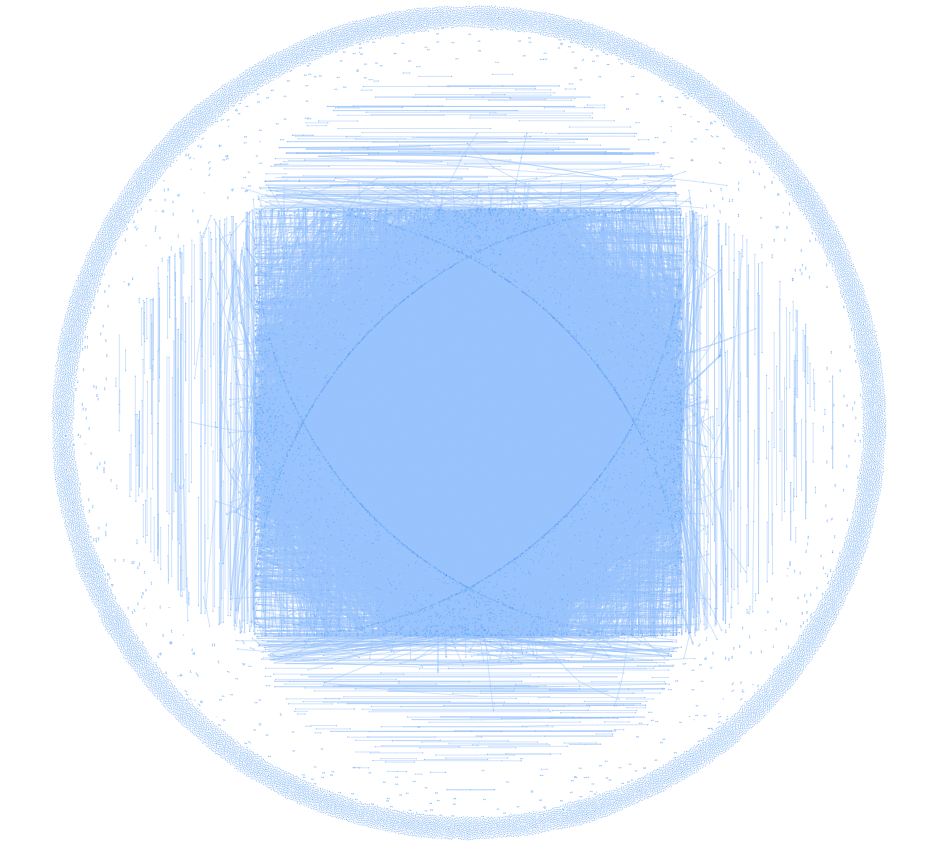
\includegraphics[width=\textwidth]{grafo-30000-completo.png}
	\caption{Grafo obtenido del Sistema Coirón. Más de 30000 personas con más casos y sus relaciones (con los siguientes criterios: involucradas en más de un caso con rol de imputado, sospechoso o denunciado; se incluyen personas fallecidas, menores y personas jurídicas)} 
	\label{fig:grafocompleto}
\end{figure}

A los sentidos prácticos de la investigación penal, una visualización con tantos nodos y relaciones no es representativa ni conduce a ningún tipo de detección de bandas delictivas, pero es un claro ejemplo del universo de datos que se disponen en el dataset utilizado, como así también la potencia de la herramienta de visualización.

También hemos incluido estadísticas resumidas en el Cuadro  \ref{tab:EstadisticasResumidas}, en donde se pueden ver la cantidad de nodos y vértices totales con los que cuenta el dataset utilizado, como así también otros parámetros interesantes de analizar para el estudio de redes sociales.

\begin{table}
	\caption{Resumen del conjunto total de datos utilizado.}\label{tab:EstadisticasResumidas}
	\centering
	\begin{tabular}{|l|r|}
		\hline
		\textbf{Característica} &  \textbf{Cantidad total} \\
		\hline
		Nodos &  33178 \\
		\hline
		Enlaces &  16964 \\
		\hline
		Relaciones Nodos/Enlaces &  60513 \\
		\hline
	\end{tabular}
\end{table}

En la Figura \ref{fig:grafosSolos} se pueden observar ejemplos en los que no se han tomado en cuenta los grupos de pertenencia de cada nodo a mostrar, es decir que sólo se visualizan las personas que pertenecen a más casos según los parámetros de búsqueda seleccionados. En la imagen (a) se muestran 10000 personas, en (b) 1000 y en (c) 100 personas con más casos.

\begin{figure}[htbp]
	\centering
	\subfigure[Top 10000.]{
		\begin{minipage}[t]{0.33\linewidth}
			\centering
			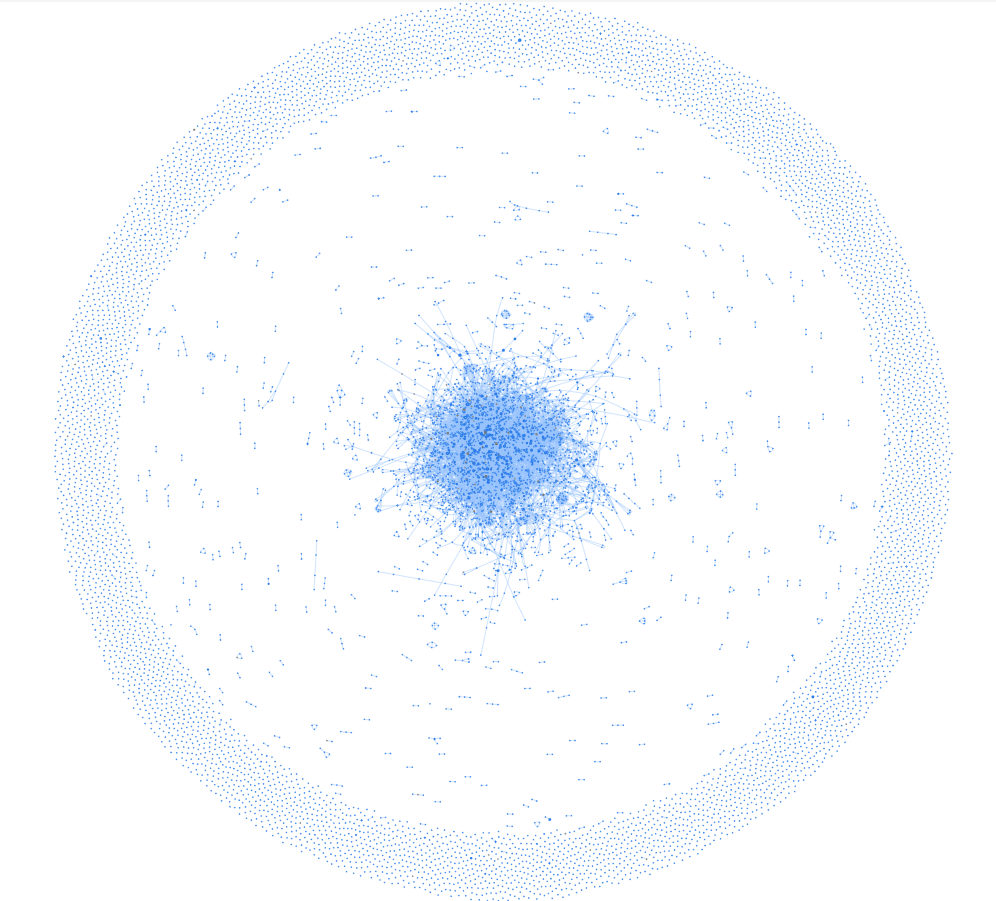
\includegraphics[width=1in]{grafo-10000-solo.png}
			%\caption{fig1}
		\end{minipage}%
	}%
	\subfigure[Top 1000.]{
		\begin{minipage}[t]{0.33\linewidth}
			\centering
			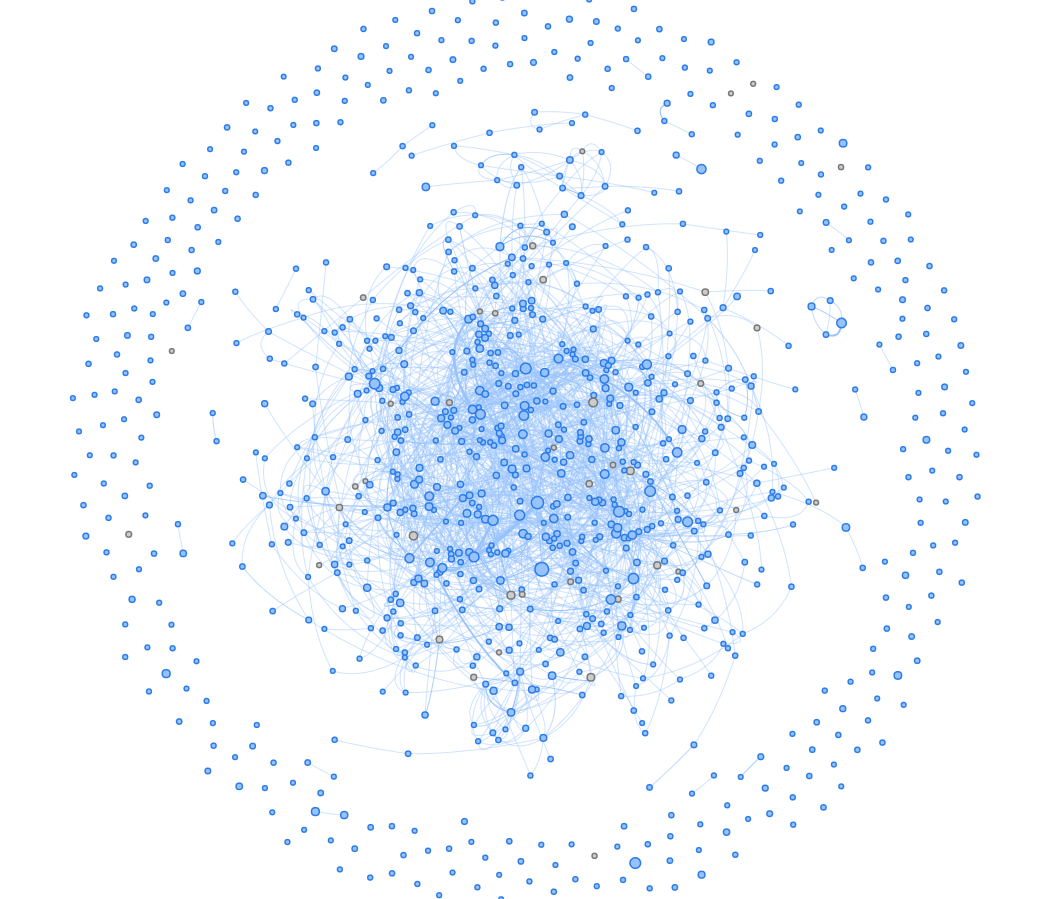
\includegraphics[width=1in]{grafo-1000-solo.png}
			%\caption{fig2}
		\end{minipage}%
	}%
	\subfigure[Top 100.]{
		\begin{minipage}[t]{0.33\linewidth}
			\centering
			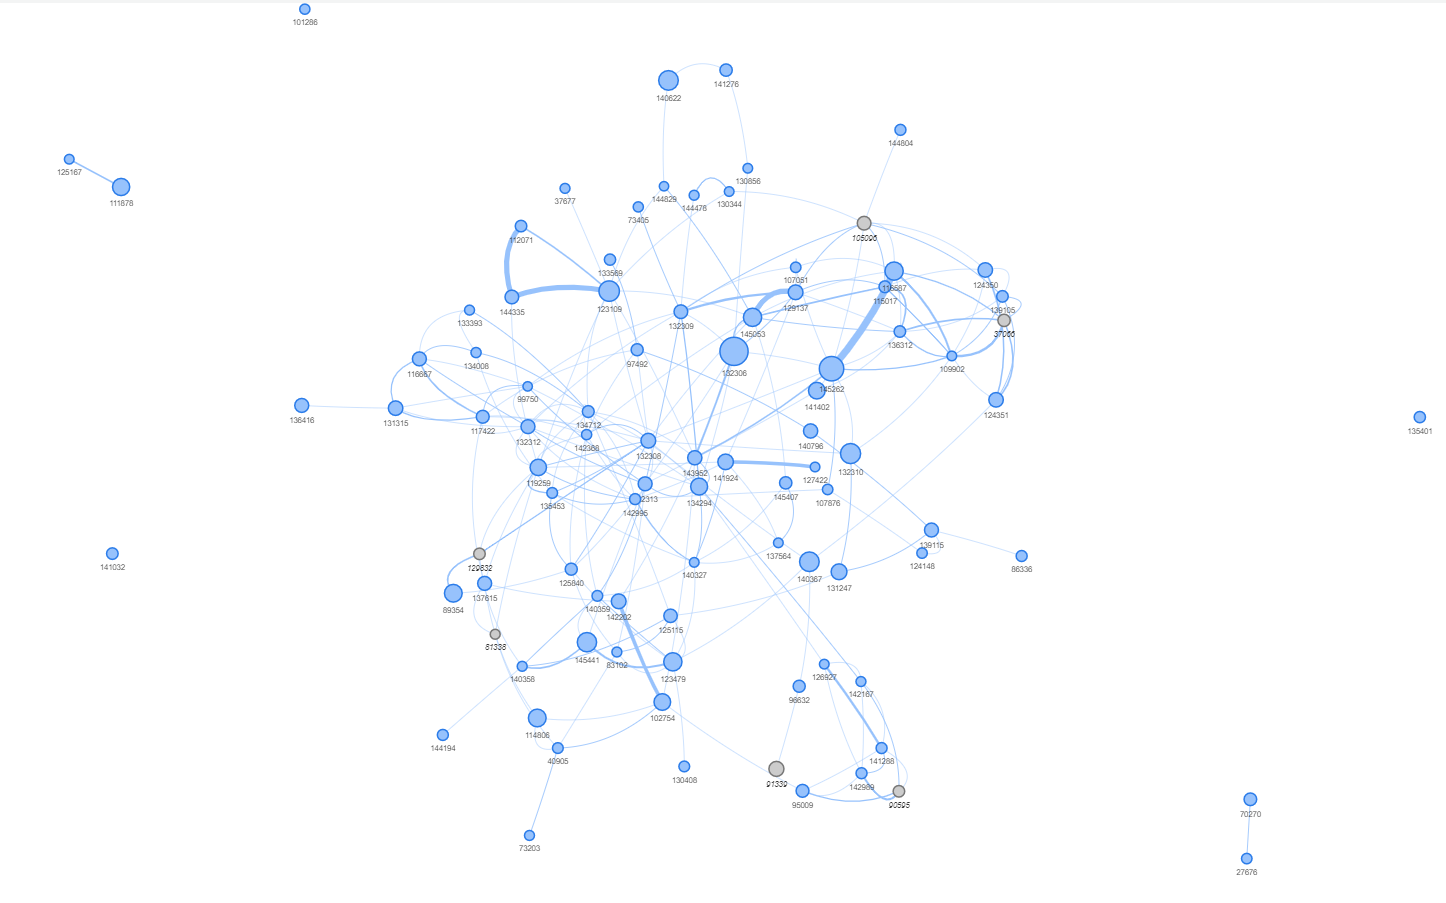
\includegraphics[width=1in]{grafo-100-solo.png}
			%\caption{fig3}
		\end{minipage}
	}%
	\centering
	\caption{ Personas en más casos, pero sin inclusión de sus grupos de pertenencia particulares.}
	\label{fig:grafosSolos}
\end{figure}

A continuación en la Figura \ref{fig:grafosCompletos} se pueden observar los mismos ejemplos que en la Figura \ref{fig:grafosSolos}, con la diferencia sustancial de que en dichas imágenes si se han tomado en cuenta los grupos de pertenencia de cada nodo. Se vuelven a visualizar las personas que pertenecen a más casos según los parámetros de búsqueda seleccionados, pero agregando para cada una de estas personas sus grupos de pertenencias particulares. En la imagen (a) se muestran 10000 personas con todos sus grupos, en (b) 1000 y en (c) 100 personas con más casos y sus grupos de pertenencia relacionados.

\begin{figure}[htbp]
	\centering
	\subfigure[Top 10000.]{
		\begin{minipage}[t]{0.33\linewidth}
			\centering
			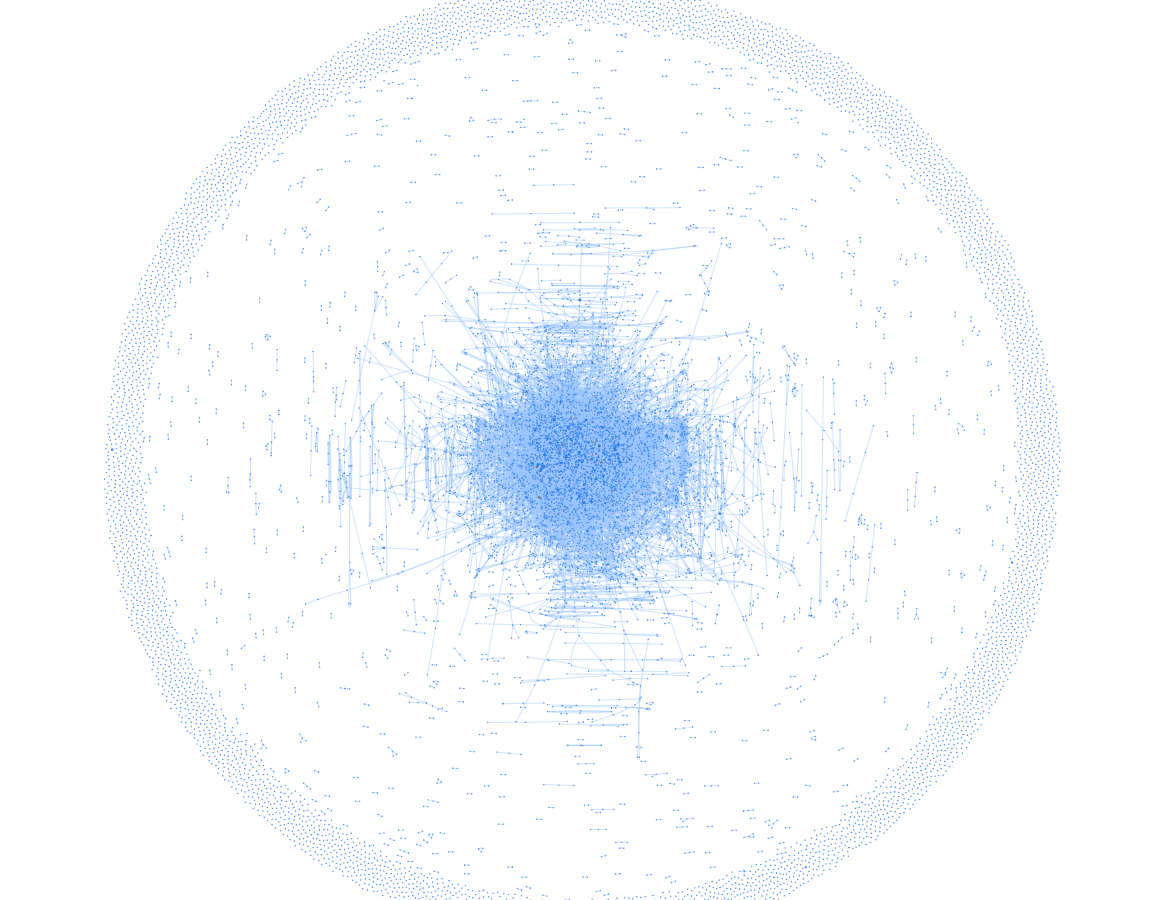
\includegraphics[width=1in]{grafo-10000-completo.png}
			%\caption{fig1}
		\end{minipage}%
	}%
	\subfigure[Top 1000.]{
		\begin{minipage}[t]{0.33\linewidth}
			\centering
			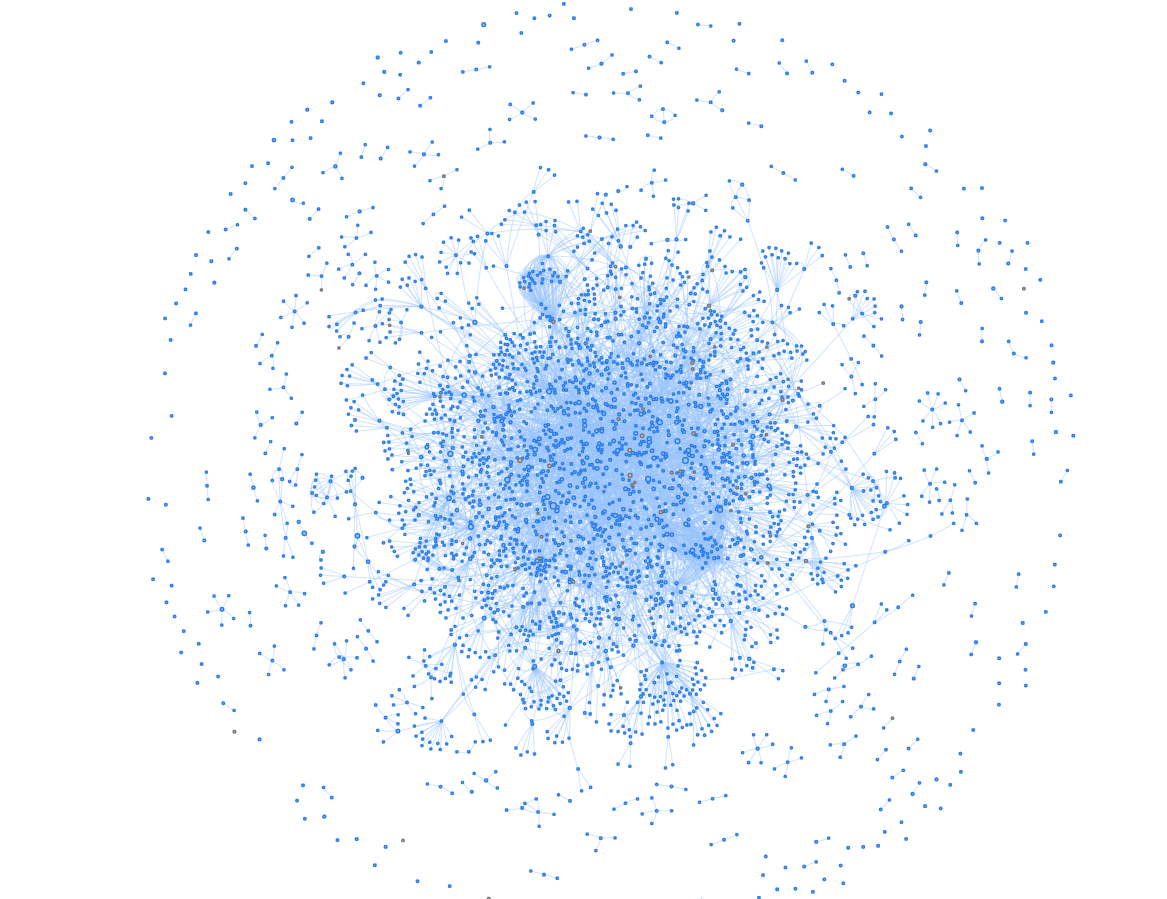
\includegraphics[width=1in]{grafo-1000-completo.png}
			%\caption{fig2}
		\end{minipage}%
	}%
	\subfigure[Top 100.]{
		\begin{minipage}[t]{0.33\linewidth}
			\centering
			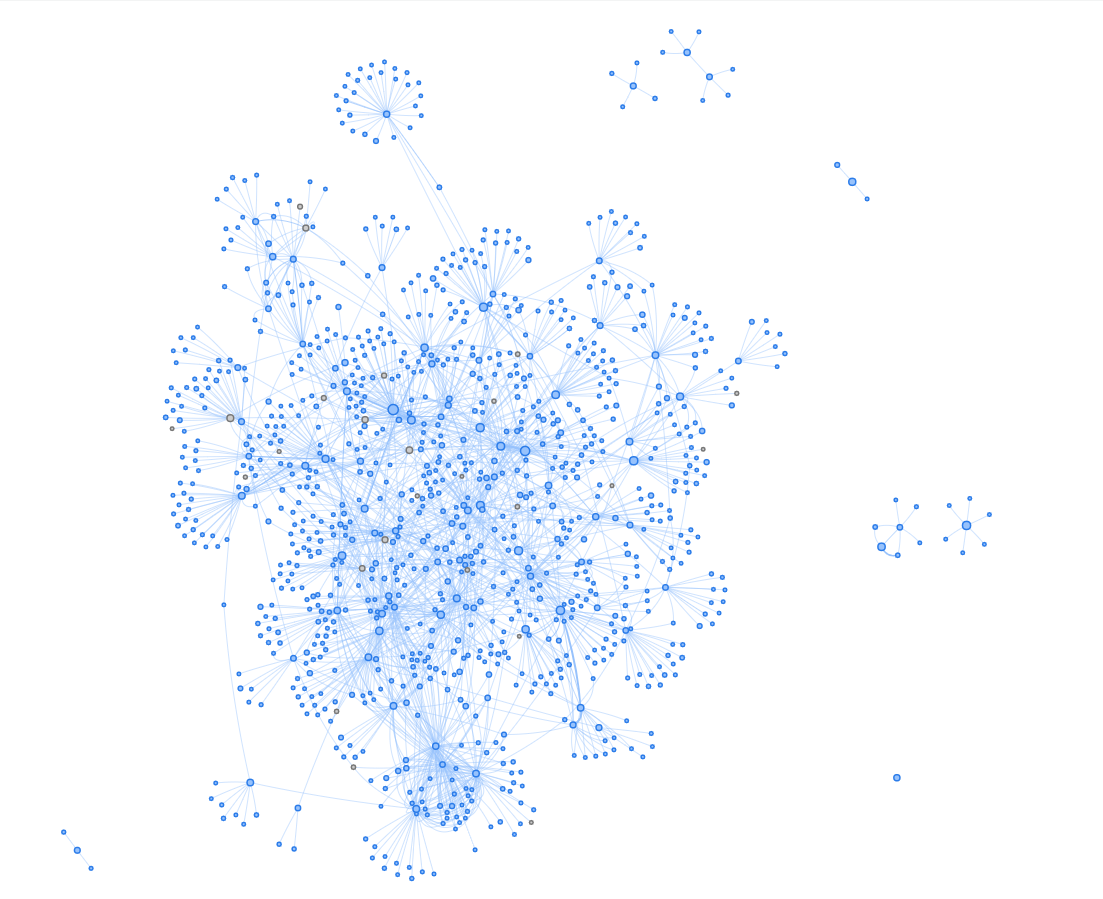
\includegraphics[width=1in]{grafo-100-completo.png}
			%\caption{fig3}
		\end{minipage}
	}%
	\centering
	\caption{ Personas en más casos, con la inclusión de sus grupos de pertenencia particulares.}
	\label{fig:grafosCompletos}
\end{figure}

Al analizar la composición de la red obtenida podemos observar las relaciones que existen entre los nodos y como se "equilibra" el grafo, haciendo que aquellos nodos con pocas o nulas relaciones queden en la periferia de la gráfica. Sumado a ello también es apreciable la medida de centralidad de aquellos nodos que son rodeados por sus relacionados.

Una aproximación más clara para denotar la medida de centralidad puede verse reflejada en la Figura \ref{fig:grafoTop10}, en donde se visualiza sólo las 10 personas con más Casos y sus grupos de pertenencia. Claramente esos 10 nodos principales quedan rodeados de sus grupos de pertenencia y se pueden observar transitividades entre ellos a través de nodos que conforman parte del grupo de pertenencia de más de un nodo principal.

\begin{figure}
	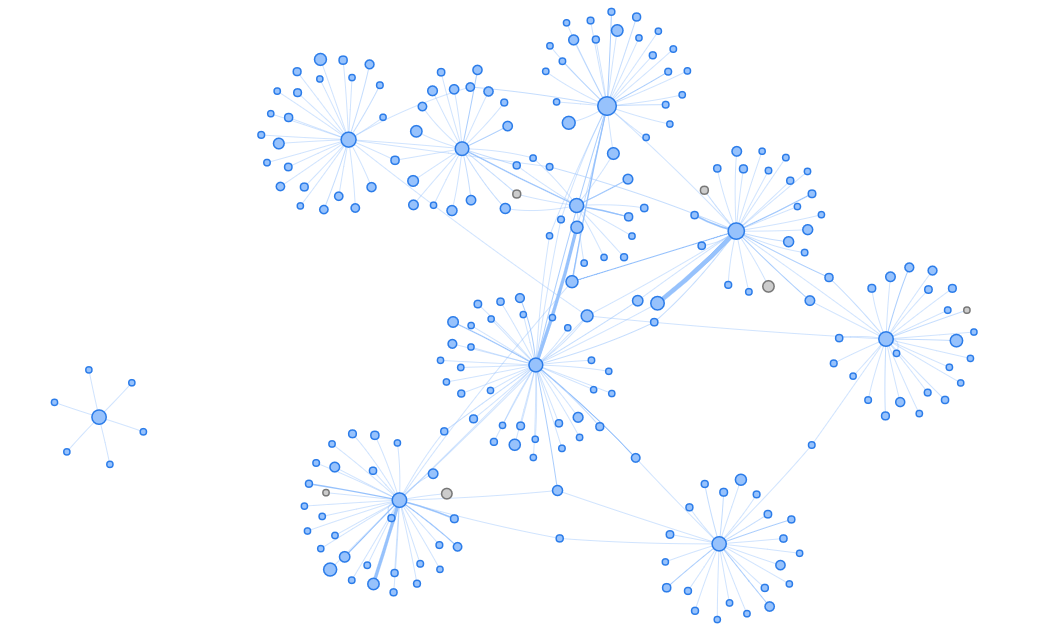
\includegraphics[width=\textwidth]{grafo-10-completo.png}
	\caption{10 personas con más casos en Coirón, con sus relaciones} 
	\label{fig:grafoTop10}
\end{figure}

Para comprender aún más de manera visual e interpretar los grupos de pertenencia de cada nodo, como así también las relaciones entre ellos, se incluye la Figura \ref{fig:grafoTop5}

\begin{figure}[htbp]
	\centering
	\subfigure[Top 5 sin grupos.]{
		\begin{minipage}[t]{0.50\linewidth}
			\centering
			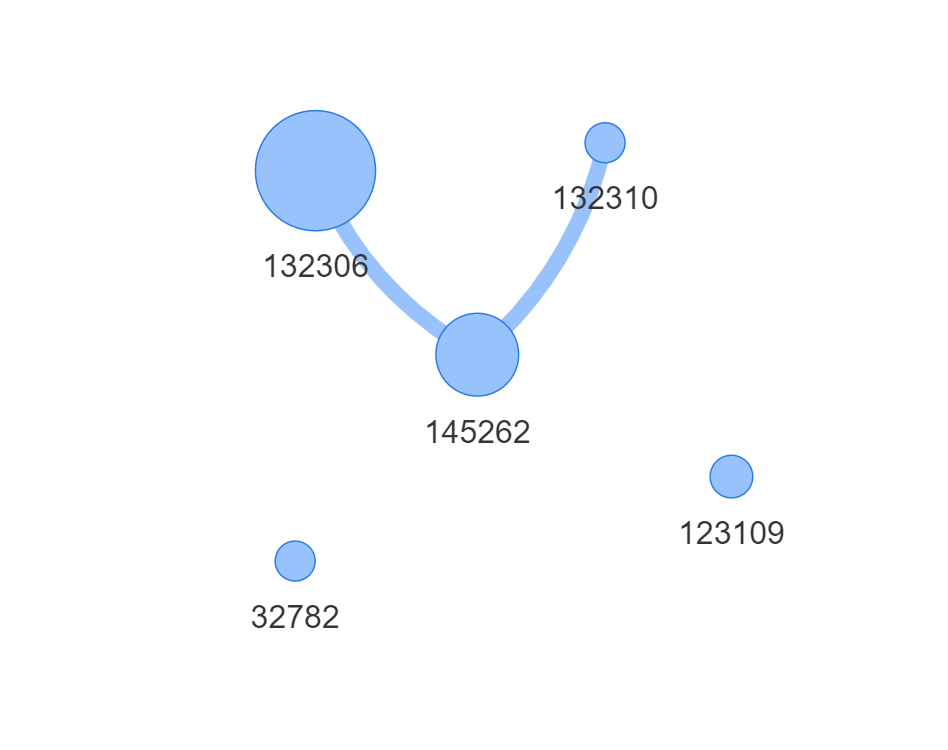
\includegraphics[width=1in]{grafo-5-solo.png}
			%\caption{fig1}
		\end{minipage}%
	}%
	\subfigure[Top 5 con grupos.]{
		\begin{minipage}[t]{0.50\linewidth}
			\centering
			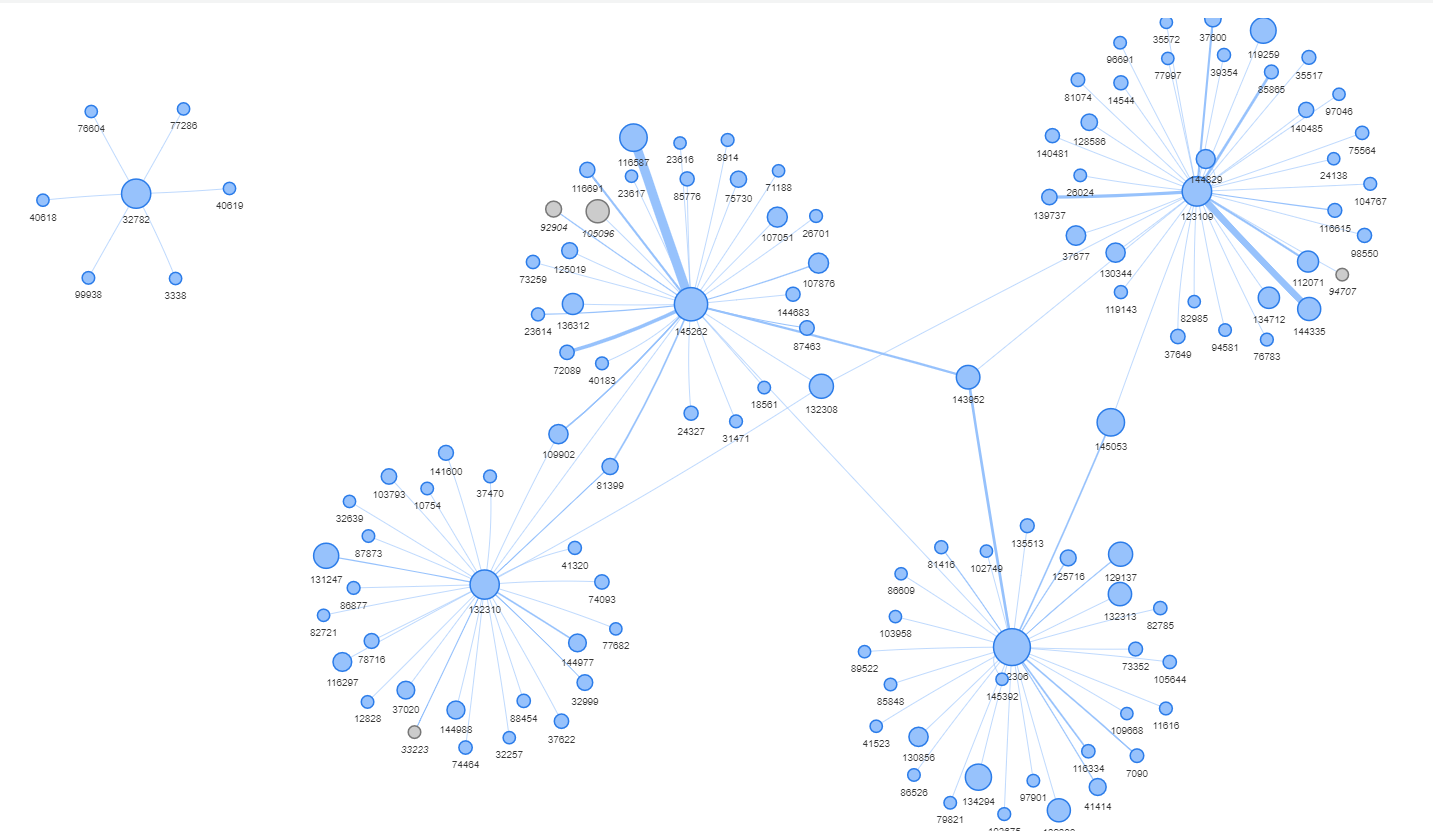
\includegraphics[width=1in]{grafo-5-completo.png}
			%\caption{fig2}
		\end{minipage}%
	}%
	\centering
	\caption{ 5 Personas en más casos. En (a) sin la inclusión de sus grupos de pertenencia particulares. En (b) con la inclusión de sus grupos de pertenencia particulares.}
	\label{fig:grafoTop5}
\end{figure}

\subsubsection{Centralidad de Grado} La centralidad de grado es una de las medidas más simples de centralidad. En esta se mide el número de enlaces o conexiones que tiene un nodo con los demás nodos pertenecientes a un grafo. Cuando se aplica un análisis de este tipo pueden determinarse diferentes medidas. Por ejemplo, en redes sociales podemos medir el grado de entrada de un nodo como la popularidad o preferencia que posea y la salida definirla como un indicador de sociabilidad. En nuestro caso de estudio, los miembros de las bandas delictivas modifican dinámicamente sus relaciones con otros miembros de la red, lo que resulta en un cambio de su rol e importancia. Una serie de medidas de centralidad de grado pueden ayudar a identificar estos cambios. Estas estadísticas se pueden utilizar para filtrar la vista de la red en función del valor de un nodo específico y resaltar su posición dentro de la red. El grado de centralidad en nuestro grafo se definirá entonces como el número de enlaces directos que tiene un delincuente. Un nodo con un alto grado puede verse como un "centro", un nodo activo e importante en la red~\cite{ref_article32}.

\subsubsection{Transitividad} El coeficiente de agrupamiento (transitividad) de un gráfico mide el grado de conexión de una red. Altos coeficientes de agrupamiento significan la presencia de un alto número de triángulos en la red. Es bien conocido en la bibliografía~\cite{ref_article34} que las redes sociales muestran valores altos del coeficiente de agrupamiento cuando reflejan la estructura social subyacente de los contactos entre amigos/conocidos. Además, los valores altos del coeficiente de agrupamiento local se consideran un indicador confiable de los nodos cuyos vecinos están muy bien conectados y entre los cuales puede fluir una cantidad sustancial de información.
